\section{Processi organizzativi}
    \subsection{Processo di coordinamento}
        \subsubsection{Introduzione processo}
            \paragraph{Descrizione}
                Questa sezione intende evidenziare quali tipologie di coordinamento e in che modi il gruppo ha deciso di organizzarsi durante l’intero svolgimento del progetto.\\ 
                Vengono specificate le modalità con cui si intratterranno le comunicazioni e le riunioni.\\
            \paragraph{Obbiettivi}
                L’obiettivo è quello di normare l’avanzamento del progetto guardando a un buon coordinamento tra i soggetti presenti all’interno del gruppo e del gruppo con i soggetti esterni al fine di ottenere un buon risultato finale.\\ 
                In questa sezione si vogliono definire le norme adottate dal gruppo per le comunicazioni e gli incontri con esterni o tra i membri del gruppo.\\
                Il processo di coordinamento è strutturato nel seguente modo:\\
                \begin{itemize}
                    \item comunicazione (interna ed esterna);
                    \item riunioni (interne ed esterne).
                \end{itemize}
        \subsubsection{Comunicazione}
            Durante lo svolgimento del progetto il gruppo EverBuilds effettuerà due tipi di comunicazioni: interne ed esterne. \\
            Le comunicazioni interne verranno fatte tra i membri del gruppo, mentre le comunicazioni esterne avverranno con il Proponente (l’azienda Zero12 rappresentata da Stefano Dindo e Michele Massaro) e con i Committenti (nella persona di prof. Tullio Vadanega e del prof. Riccardo Cardin).\\
            \paragraph{Comunicazione interna}
                Le comunicazioni interne al gruppo avvengono utilizzando il software di messaggistica: Telegram, le sue funzionalità e la sua comodità ne hanno indotto la scelta.
            \paragraph{Comunicazione esterna}
                Le comunicazioni con i soggetti esterni saranno di competenza del Responsabile di Progetto, che parlerà a nome dell’intero gruppo, attraverso un indirizzo di posta elettronica creato appositamente. L’email utilizzata sarà: \url{everbuilds12@gmail.com} .
                Si ritiene opportuno che le e-mail inviate presentino una struttura predefinita:
                \begin{itemize}
                    \item\textbf{Oggetto}: l’oggetto della mail preceduto dalla sigla “[SWE UNIPD]” per far si che sia chiaro l’ambito di riferimento della mail;
                    \item\textbf{Corpo}: il contenuto dovrà essere scritto con un tono formale e dovrà essere sintetico ed esaustivo per far si che il problema e/o le eventuali richieste in questione siano esposte nel miglior modo possibile.
                \end{itemize}
                Ogni membro del gruppo possiede le credenziali per poter accedere all’indirizzo email del gruppo.\\
                Per comunicare con l’azienda Zero12 in un modo più efficiente si utilizza un canale Slack per la chat testuale.
        \subsubsection{Riunioni}
            Questa sezione serve per definire le modalità con cui verranno effettuate le riunioni interne ed esterne del gruppo. \\
            Per ogni riunione sarà nominato un segretario che avrà il compito di far rispettare l’ordine del giorno e di tener traccia della discussione effettuata per poter poi redigere il \dext{Verbale} della riunione.\\
            Il \dext{Verbale} della riunione verrà redatto seguendo le norme alla sezione 3.2.5.3.1 .\\
            \paragraph{Riunioni interne}
                La partecipazioni alle riunioni interne è permessa solo ai membri del gruppo.        \\
                Durante le riunioni verranno prese delle decisioni che dovranno avere la maggioranza dei voti.\\
                Perchè una riunione sia valida il Responsabile di Progetto dovrà fissare preventivamente la data della riunione, previa disponibilità della maggior parte dei componenti del gruppo, stabilire un ordine del giorno, nominare un segretario per l’incontro e approvarne il \dext{Verbale}.\\
                I partecipanti alla riunione dovranno avvertire preventivamente in caso di assenza e altrimenti essere puntuali all’orario stabilito e partecipare alla discussione.\\
                Le riunioni interne verranno effettuate tramite video-chiamata sulla piattaforma Discord al canale creato appositamente per il gruppo EverBuilds. È stato preferito ad altri servizi per la sua versatilità, il fatto di essere open-source e perché multi-piattaforma.\\
            \paragraph{Riunioni esterne}
                Alle riunioni esterne dovranno partecipare tutti i membri del gruppo ed i soggetti esterni, quali il proponente ed i committenti.\\
                Il Responsabile di Progetto ha il compito di organizzare gli incontri con il proponente ed i committenti, dovrà decidere una data in accordo con tutte le parti e comunicarla ai vari partecipanti tramite i canali predefiniti.\\
                Anche per le riunioni esterne è prevista la nomina di un segretario che dovrà redigere il \dext{Verbale} dell’incontro.\\
                Le riunioni esterne verranno effettuate utilizzando Google Meet.\\
        \subsubsection{Strumenti}
            \begin{itemize}
                \item \href{https://discordapp.com/company/}{Discord}
                \item \href{https://www.google.com/intl/it/gmail/about/}{Gmail }
                \item \href{https://meet.google.com/?hs=197\&pli=1\&authuser=0}{Google Meet}
            \end{itemize}
    \subsection{Processo di pianificazione}
        \subsubsection{Introduzione processo}
            \paragraph{Descrizione}
                Questa sezione mette in luce i processi di pianificazione ossia i vari ruoli presenti all’interno del progetto e come avverrà l’assegnazione dei compiti ai vari membri del team. 
            \paragraph{Obbiettivi}
                L’obiettivo è quello di normare la suddivisione dei vari ruoli, con i relativi compiti, in modo da poterli assegnare adeguatamente. Si vuole chiarire quali saranno le mansioni di ciascun ruolo, come verranno assegnati i ruoli ai vari partecipanti e qual è il ciclo di vita del ticket.
        \subsubsection{Ruoli di progetto}
            \paragraph{Responsabile di progetto}
                Il responsabile di progetto è un ruolo fondamentale in quanto rappresenta il progetto ed è presente come figura per tutta la durata del lavoro. Rappresenta il gruppo presso il proponente e i committenti e ne presenta i risultati del lavoro svolto. Il suo compito principale è quello di coordinare l’intera struttura e organizzare il lavoro avendo responsabilità di scelta e approvazione per ottenere uno sforzo utile al fine comune.\\
                Questo ruolo ha la responsabilità di: \\
                \begin{itemize}
                    \item pianificare le attività da svolgere e coordinare i membri del gruppo controllando che quanto assegnato a ciascuno venga portato a termine rispettando le scadenze;
                    \item    si occupa delle risorse umane e dell’assegnazione dei ruoli garantendo che vengano rispettati;
                    \item    responsabile della stima dei costi e dell’analisi e gestione dei rischi;
                    \item    deve curare le relazioni che il gruppo intratterrà con i soggetti esterni;
                    \item deve approvare i documenti;
                    \item assicurarsi che l’attività di verifica e validazione vengano svolte sistematicamente.
                \end{itemize}
            \paragraph{Amministratore }
                L’Amministratore di Progetto è incaricato di gestire, controllare e curare gli strumenti che il gruppo utilizza per svolgere il proprio lavoro. \\
                È la figura che garantisce l’affidabilità, l’efficienza e l’efficacia dei mezzi scelti dal gruppo e del rendimento dell’ambiente di lavoro pertanto deve:\\
                \begin{itemize}
                    \item amministrare infrastrutture e servizi necessari ai processi di supporto;
                    \item gestire il versionamento e la configurazione dei prodotti;
                    \item gestire la documentazione di progetto, controllando che venga corretta, verificata ed approvata, e facilitandone il reperimento;
                    \item correggere eventuali problemi relativi alla gestione dei processi e alle difficoltà di controllo;
                    \item individuare strumenti utili all’automazione del maggior numero possibile di compiti e operazioni.
                \end{itemize}
                L’amministratore dirige la redazione delle \dext{Norme di Progetto} v1.0.0 nelle quali norma l’utilizzo di strumenti e redige anche il \dext{Piano di Qualifica} v1.0.0 in cui si descrivono strumenti e metodi di verifica.
            \paragraph{Analista}
                L’Analista partecipa al progetto soprattutto nelle sue fasi iniziali quando si redige il documento \dext{Analisi dei Requisiti} v1.0.0. Il suo compito è quello di comprendere appieno la natura e complessità del problema evidenziandone i punti chiave. \\
                È fondamentale per la buona riuscita del lavoro perché errori o mancanze nell’individuazione dei requisiti potrebbero compromettere la successiva attività di progettazione.\\
                Le sue mansioni sono:\\
                \begin{itemize}
                    \item studiare e definire il problema;
                    \item analizza le richieste e definisce quali sono i requisiti studiando i bisogni, siano essi impliciti o espliciti;
                    \item analizza il fronte applicativo, in particolare gli utenti e i casi d’uso;
                    \item produce una specifica di progetto motivata e comprensibile dal proponente, dal committente e dai progettisti.
                \end{itemize}
                L’analista inoltre redige i documenti: \dext{Studio di Fattibilità} v1.0.0 e \dext{Analisi dei Requisiti} v1.0.0.
            \paragraph{Progettista }
                Il Progettista parte dal lavoro svolto dall’Analista, e ha il compito di sviluppare una soluzione che soddisfi i bisogni individuati. Questa figura è responsabile delle attività di progettazione infatti il suo scopo è quello di produrre un’architettura che modelli il problema a partire da un insieme di requisiti. \\
                Le mansioni di questo ruolo sono le seguenti:\\
                \begin{itemize}
                    \item effettuare scelte su aspetti di progettazione applicando principi noti e collaudati per produrre un’architettura che assicuri coerenza e consistenza anche per una mantenibilità nel tempo;
                    \item deve produrre una soluzione sostenibile e realizzabile, che rientri nei costi stabiliti dal preventivo;
                    \item si adopera per la costruzione di una struttura che soddisfi tutti i requisiti e che sia comprensibile e motivata;
                    \item cerca di limitare il più possibile il grado di accoppiamento tra le varie componenti;
                    \item rivolge il suo sforzo verso la ricerca dell’efficienza, dell’affidabilità, della flessibilità e della riutilizzabilità.
                \end{itemize}
            \paragraph{Programmatore }
                Il Programmatore è la figura incaricata delle attività di codifica e delle componenti necessarie per effettuare le prove di verifica. Egli deve implementare l’architettura prodotta dal Progettista in maniera che aderisca alle specifiche, ed è responsabile della manutenzione del codice creato. \\
                Egli:
                \begin{itemize}
                    \item codifica secondo le specifiche stabilite dal Progettista. Il codice scritto deve essere documentato, versionato, mantenibile ed deve essere strutturato in modo che rispetti le metriche stabilite per la scrittura;
                    \item implementa i test che serviranno poi per la verifica e la validazione del codice;
                    \item scrive il Manuale Utente relativo al codice prodotto.
                \end{itemize}
            \paragraph{Verificatore  }
                Il Verificatore è il responsabile delle attività di verifica ed è presente per tutta la durata del progetto. \\
                I compiti del Verificatore sono:\\
                \begin{itemize}
                    \item occuparsi di controllare che le attività svolte rispettino le norme e le attese prefissate;
                    \item controllare ed accertarsi che l’esecuzione delle attività di processo non abbia causato errori;
                    \item redigere la parte retrospettiva del \dext{Piano di Qualifica} v1.0.0, la quale illustra l’esito e la completezza delle verifiche e delle prove effettuate;
                    \item svolgere l’attività di analisi dei problemi accidentali riportati dal Responsabile del progetto.
                \end{itemize}
        \subsubsection{Assegnazione dei compiti}
            L’avanzamento nello svolgimento del progetto è visto come il completamento di una serie di compiti in maniera sequenziale o parallela. \\
            Ogni compito ha una scadenza temporale e l’insieme di tutte le mansioni svolte porta a dei risultati utili per il completamento degli obiettivi prefissati.\\
            Si è deciso di utilizzare il servizio di ticketing di GitHub basato su issue per l’assegnazione di compiti.\\
            La gestione dei compiti è affidata al Responsabile di Progetto che dovrà individuare il compito da svolgere (se troppo complesso suddividerlo), individuare uno o più componenti del gruppo al quale assegnarlo ed infine aprire una issue ed affidare il compito al soggetto/i selezionato/i definendo la data di scadenza entro cui dovrà essere svolto.\\
            I membri del gruppo dovranno impegnarsi a svolgere e completare i compiti a loro assegnati entro la scadenza prestabilita e saranno loro i responsabili della chiusura della issue quando avranno terminato il lavoro.\\
        \subsubsection{Ciclo di vita dei ticket}
            I soggetti che sono presenti dal momento dell’individuazione del compito da svolgere fino al suo completamento sono 3:
            \begin{itemize}
                \item\textbf{Responsabile di progetto}: sarà colui che si occuperà di individuare la mansione da eseguire, determinare a chi verrà assegnata e successivamente aprire la issue relativa. Quanto il lavoro sarà terminato e verificato dovrà approvarlo;
                \item\textbf{Assegnatario}: membro del gruppo a cui verrà dato il compito di completare un lavoro;
                \item\textbf{Verificatore}: persona incaricata di controllare e verificare il lavoro svolto dall'Assegnatario. Nel caso il lavoro non verrà ritenuto valido ha la facoltà di riaprire la issue.
            \end{itemize}
            Indipendentemente dalla natura del compito da svolgere il ciclo di vita del ticket sarà il seguente:
            \begin{itemize}
                \item\textbf{individuazione del compito}: il Responsabile di Progetto nel momento in cui rileverà delle necessità, che dovranno essere soddisfatte con opportune azioni, le identificherà con delle richieste da soddisfare ed obiettivi da raggiungere creando così un compito;
                \item\textbf{analisi del compito}: il Responsabile di Progetto dovrà analizzare il compito appena identificato per stimare la sua complessità e in caso questa sia elevata lo potrà suddividere in vari sotto-compiti. A questo punto individuerà uno o più soggetti del gruppo che diventeranno gli Assegnatari e stabilirà una data di scadenza entro cui il lavoro dovrà essere svolto;
                \item\textbf{creazione issue}: il Responsabile di Progetto creerà ora una issue utilizzando GitHub definendo l’Assegnatario e la data di scadenza;
                \item\textbf{spostamento issue in TO-DO}: quando la issue sarà creata il Responsabile avrà il compito di spostarla nella sezione “TO-DO” della dashboard del progetto dove saranno presenti tutti i compiti individuati ma non ancora svolti; 
                \item\textbf{spostamento della issue in IN PROGRESS}: quando l’Assegnatario inizierà il lavoro dovrà spostare la issue nella sezione “IN PROGRESS”;
                \item\textbf{svolgimento issue}: l’Assegnatario in questo periodo di tempo dovrà portare a termine il lavoro a lui assegnato utilizzando adottando la strategia dei feature branch;
                \item\textbf{pull request}: Una volta svolto il proprio compito, l'assegnatario dovrà avviare il processo di pubblicazione di una pull request, questo per notificare gli interessati alla verifica del documento;
                \item\textbf{verifica del lavoro}: a questo punto il Verificatore avrà il compito di verificare il lavoro svolto dall’Assegnatario e potrà accettare il lavoro svolto o altrimenti rifiutare quanto fatto spostando nuovamente la issue nella sezione “TO-DO”. Vedi attività di verifica sezione §3.5 ;
                \item\textbf{approvazione del lavoro}: il Responsabile di progetto esaminerà ulteriormente il lavoro eseguito, controllando che rispetti effettivamente gli obiettivi prefissati inizialmente, e lo approva;
                \item\textbf{spostamento issue in DONE}: quando il lavoro sarà completato l’Assegnatario avrà il compito di spostare la issue nella sezione “DONE”.
            \end{itemize}
            Il ciclo di vita del ticket è rappresentato graficamente dal seguente diagramma delle attività
            \begin{figure}[H]
                    \centering
                    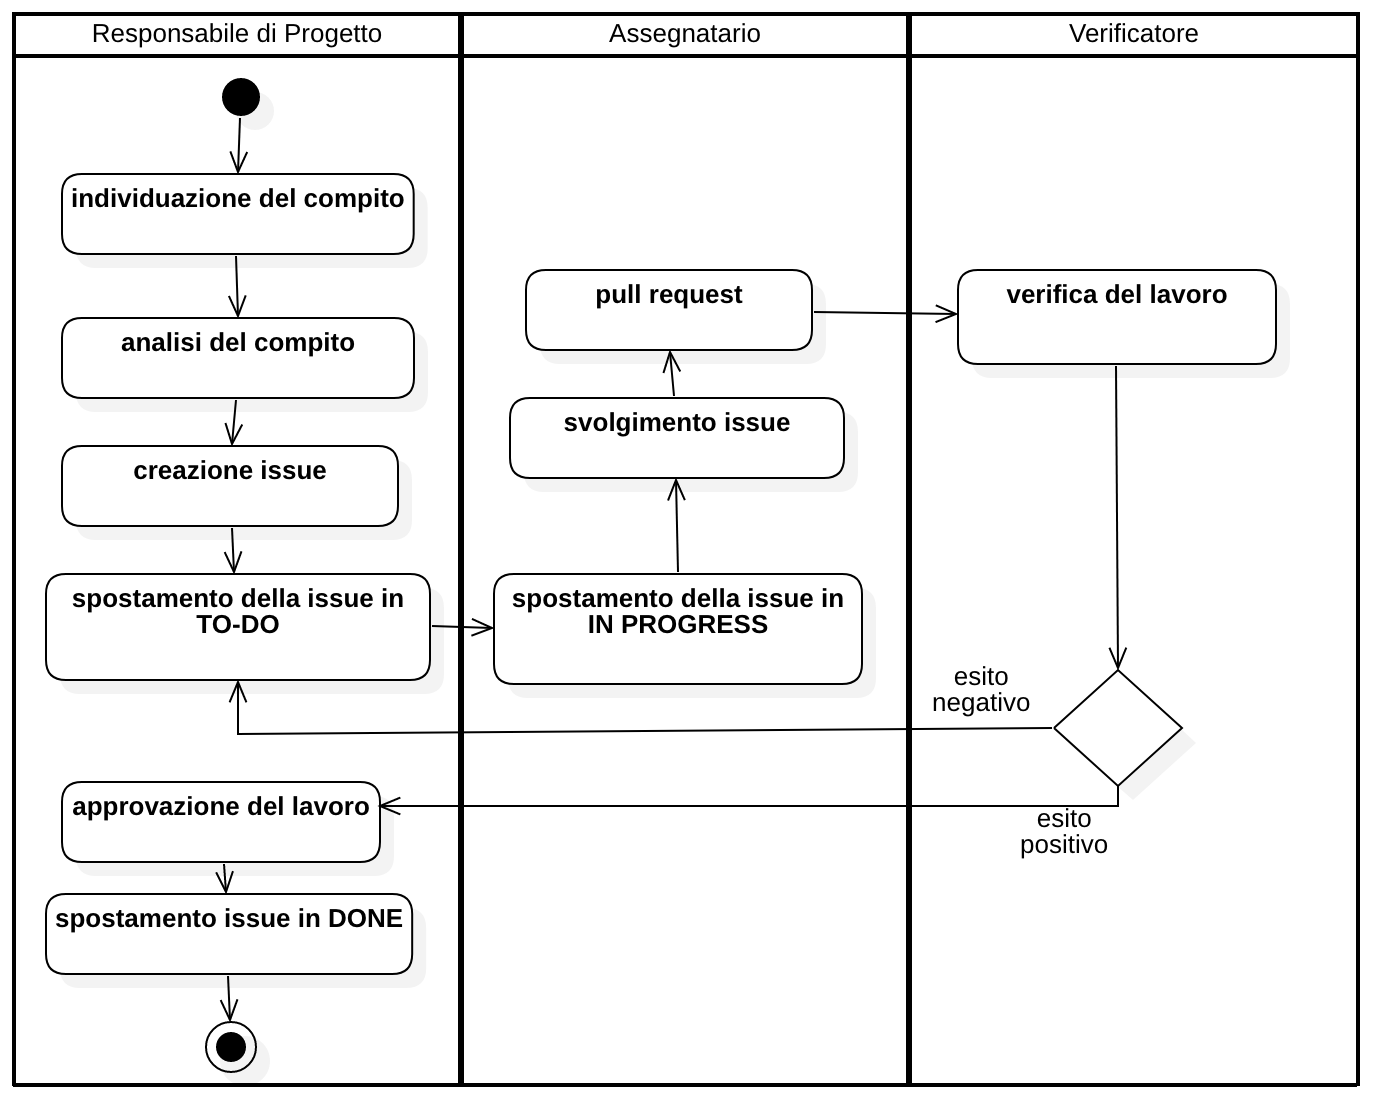
\includegraphics[width=1.0\textwidth]{res/images/ciclo_di_vita_del_ticket.png}
                \caption{Ciclo di vita del ticket}
                \label{Ciclo di vita del ticket}
            \end{figure}
        \subsubsection{Metriche}
            La presente sezione espone le metriche selezionate dal gruppo per misurare il raggiungimento degli obiettivi di qualità del processo di Pianificazione.
            \paragraph{Gestione della spesa }
                Si vuole gestire la copertura di risorse disponibili per la realizzazione del progetto, monitorando i costi aggiuntivi e le tempistiche non rispettate dalla pianificazione prevista.\\
                Per la gestione delle risorse si farà uso delle seguenti metriche:
                \begin{itemize}
                    \item\textbf{QM-PC-PNF01 Budgeted cost of work scheduled (BCWS)}
                        \begin{itemize}
                            \item\textbf{Descrizione}: la metrica BCWS definisce il costo pianificato per realizzare le attività di progetto alla data corrente;
                            \item\textbf{Unità di misura}: in EURO.
                        \end{itemize}
                    \item\textbf{QM-PC-PNF02 Actual cost of work performed (ACWP)}
                        \begin{itemize}
                            \item\textbf{Descrizione}: la metrica ACWP definisce il costo effettivamente sostenuto per realizzare le attività di progetto alla data corrente;
                            \item\textbf{Unità di misura}: in EURO.
                        \end{itemize}
                    \item\textbf{QM-PC-PNF03 Budgeted cost of work performed (BCWP)}
                        \begin{itemize}
                            \item\textbf{Descrizione}: la metrica BCWP definisce il valore delle attività realizzate alla data corrente. In altre parole, misura il valore del prodotto fino ad ora realizzato;
                            \item\textbf{Unità di misura}: in EURO.
                        \end{itemize}
                    \item\textbf{QM-PC-PNF04 Schedule variance (SV)}
                        \begin{itemize}
                            \item\textbf{Descrizione}: la metrica SV indica se si è in anticipo, in ritardo o in linea rispetto alle schedulazioni pianificate per il progetto. Questo può essere utile per il cliente per valutare l'efficacia del gruppo nei confronti della realizzazione del progetto;
                            \item\textbf{Unità di misura}: percentuale;
                            \item\textbf{Formula}: \\
                                \[SV = \frac{\mathit{BCWP} - \mathit{BCWS}}{\mathit{BCWS}} \times 100\]
                            \item\textbf{Risultato}:
                                \begin{itemize}
                                    \item un risultato positivo (>0) indica che il progetto è avanti rispetto alla schedulazione;
                                    \item un risultato negativo (<0) indica che il progetto è indietro rispetto alla schedulazione;
                                    \item un risultato pari a zero (=0) indica che il progetto è in linea rispetto alla schedulazione.
                                \end{itemize}
                        \end{itemize}
                    \item\textbf{QM-PC-PNF05 Cost variance (CV)}
                        \begin{itemize}
                            \item\textbf{Descrizione}: la metrica CV indica se il valore del costo realmente maturato è maggiore, minore o uguale rispetto al costo effettivo. In altre parole, permette di comprendere con che livello di efficienza il gruppo sta sviluppando il progetto, rispetto a quanto pianificato;
                            \item\textbf{Unità di misura}: percentuale;
                            \item\textbf{Formula}: \\
                                \[CV = \frac{\mathit{BCWP} - \mathit{ACWP}}{\mathit{BCWP}} \times 100\]
                            \item\textbf{Risultato}:
                                \begin{itemize}
                                    \item un risultato positivo (>0) indica che il progetto sta sviluppando con un costo minore rispetto a quanto pianificato (maggiore efficienza);
                                    \item un risultato negativo (<0) indica che il progetto sta sviluppando con un costo maggiore rispetto a quanto pianificato (minore efficienza);
                                    \item un risultato pari a zero (=0) indica che il progetto sta sviluppando con un costo in linea rispetto a quello pianificato.
                                \end{itemize}
                        \end{itemize}
                \end{itemize}
            \paragraph{Gestione dei rischi}
                Nel contesto della gestione dei rischi legati allo svolgersi delle attività del progetto, definiamo delle metriche che mirano a dare una valenza quantitativa dei possibili inconvenienti. Così facendo andiamo a tracciare la loro influenza nel progetto e nella prospettiva dei suo futuro a breve e medio termine.\\
                Per la gestione dei rischi si farà uso delle seguenti metriche:
                \begin{itemize}
                    \item\textbf{QM-PC-PNF06 Unbudgeted risks (UR)}
                        \begin{itemize}
                            \item\textbf{Descrizione}: la metrica UR viene utilizzata per tracciare in modo incrementale tutti i nuovi rischi non precedentemente preventivati che si presentano durante una fase del progetto;
                            \item\textbf{Unità di misura}: valore intero che parte da 0;
                            \item\textbf{Formula}: per ogni rischio non preventivato e non individuato precedentemente che viene rilevato, si incrementa di una unità il numero di rischi rilevati fino alla data corrente, a partire da una fase del progetto
                                \[UR = UR + 1 \]
                            \item\textbf{Risultatot}:
                                \begin{itemize}
                                    \item un valore pari a 0, indica che non sono stati trovati rischi nella fase del progetto;
                                    \item un valore superiore a 0, indica che sono stati trovati rischi nella fase del progetto.
                                \end{itemize}
                        \end{itemize}
                \end{itemize}
    \subsection{Formazione}
        \subsubsection{Introduzione processo}
            \paragraph{Descrizione}
                Il processo di Formazione è il processo che deve interessare singolarmente ciascun membro del gruppo e consiste nell’apprendere le competenze e le conoscenze necessarie allo svolgimento delle attività che è tenuto a svolgere.
            \paragraph{Obbiettivi}
                L'obiettivo è provvedere alla formazione in maniera autonoma studiando le tecnologie utilizzate e/o colmando eventuali lacune.
        \subsubsection{Tecnologie e linguaggi per formazione}
            Si invitano i membri del gruppo a visionare i documenti riferiti alla sezione §1.4.2 .
        \subsubsection{Condivisione del Know How}
            I membri del gruppo che apprendono una nuova tecnologia sono spronati a condividere un qualunque forma ritengano opportuna le conoscenze apprese agli altri membri del gruppo che non la conoscono e con cui dovranno interfacciarsi in futuro.




            
            
            
            
            
            
            
            
            
            
            
            
            
            
            
            